\documentclass[openright]{nitocs}
% \documentclass[openright,draft]{nitocs} % draftを入れると画像が表示されない.下書き時のコンパイル短縮用

%\documentclass[interim]{nitocs}

% \usepackage[dvipdfmx]{graphicx}
\usepackage[dvipdfmx]{graphicx}
\usepackage{latexsym}
\usepackage{listings}
\usepackage{bm}

% 数式番号記述
\usepackage{amsmath}
\numberwithin{equation}{section}
\graphicspath{{./IMG/}} % 画像指定用のパス

\renewcommand{\theequation}{\arabic{equation}}
\renewcommand{\thefigure}{\arabic{section}.\arabic{figure}}
\renewcommand{\thetable}{\arabic{section}.\arabic{subsection}.\arabic{table}}
\makeatletter
\@addtoreset{equation}{section}
\@addtoreset{figure}{section}
\@addtoreset{table}{section}
\setlength{\mathindent}{0pt}
% 
\def\Underline{\setbox0\hbox\bgroup\let\\\endUnderline}
\def\endUnderline{\vphantom{y}\egroup\smash{\underline{\box0}}\\}
\def\|{\verb|}

\setcounter{page}{1}
\begin{document}

    \title{囲碁における碁石識別システムの検討}  % タイトル
    \etitle{A Study of System for Extracting Go Stone Positions}  % 英語タイトル
    \author{橋本 燎}{Ryo Hashimoto} % 氏名
    \advisor{井上 優良}{Yusuke Inoue}   % 指導教員氏名
    % \date{令和3年1月dd日}   % 日付
    \date{令和3年\number\month 月\number\day 日} %! 実行時の日付が自動挿入されるはず

    \begin{abstract} % 概要
        本研究では,人間の手による記録をなくしてコンピュータが単独で囲碁の戦局を把握できるように,囲碁盤の画像から碁石の配置を識別するシステムを検討する.
        システムは,指定した四隅の座標をもとに碁盤を切り抜き,グレースケール変換を行った後に,石を設置できる座標の色情報から石の検出を行う.
        実際の画像にシステムを適用した結果,石の位置がずれている,盤面が光を反射している等がない場合に限り,碁石の配置を正常に識別することができた.
    \end{abstract}

    \begin{keyword} % キーワード
        画像処理,OpenCV,射影変換,メディアンフィルタ
    \end{keyword}


    \maketitle

    % セクション.序論
    % https://www.google.com/url?sa=t&rct=j&q=&esrc=s&source=web&cd=&ved=2ahUKEwj58aT9i4ruAhXTZt4KHcLBBQIQFjAGegQICRAC&url=https%3A%2F%2Fipsj.ixsq.nii.ac.jp%2Fej%2F%3Faction%3Drepository_action_common_download%26item_id%3D90404%26item_no%3D1%26attribute_id%3D1%26file_no%3D1&usg=AOvVaw2sTiUa2iijA6FG63LerTuI
    \section{緒言}  
    \label{sec:format}
            % 前書き
            % 囲碁・棋譜について(もうちょっと説明が欲しい,けど書くことが無い)
        囲碁は,2人のプレイヤーが碁石を碁盤へ配置するボードゲームである.碁石は各プレイヤーが使用する白黒の石であり,碁盤は通常$19\times19$の格子状の盤面のことを指す.
        %! ルール説明とかで文章を増やそう
        このゲームは両プレイヤーが碁石を交互に碁盤上に設置し,碁石で囲まれた陣地を多く確保したプレイヤーが勝利する.
        相手の陣地として成立している領域でなければどこにでも碁石を置くことができる,相手プレイヤーの碁石を陣地内に収めることでその碁石を奪い使用することで相手陣地の縮小を行うことができる等,
        ルール上の制約が極めて少ないといった特徴を持つため,他のボードゲームと比較すると可能な総局面数は膨大になる.
        2016年には$19\times19$の盤面における総局面数の正確な値が計算され,約$2.081681994 \times 10^{170}$通りということが明らかにされた\cite{numbers}.
        これはオセロや将棋の総局面数を超え,観測可能な宇宙に存在する原子の総数(約$4\times10^{79}$個)よりも遥かに大きな値である.

            % ここもっと書きたい.コンピュータと囲碁の関係とか.最近AIとかで盛んになってきてることとか.(ただ良さげな参考文献が無い!!)
            % 『コンピュータ囲碁研究』(https://www.jstage.jst.go.jp/article/jjsai/10/6/10_860/_pdf/-char/ja)
        コンピュータの世界において,囲碁の研究は1960年代から行われていた.
        最も古い研究は,1962年のRemusによる研究\cite{Remus}とされている.
        1969年にはZobristが世界で初めて囲碁が動作するコンピュータプログラムを作った\cite{Zobrist}.
        2005年には,膨大な局面数における最適な行動を決定するために,モンテカルロ木探索を実装した囲碁プログラム{\it Crazy Stone}\cite{CrazyStone}が開発された.
        これは様々な大会で優秀な成績を記録し,以降のコンピュータ囲碁プログラムでも同様のアルゴリズムを採用するなど,コンピュータ囲碁の研究開発に大きな進歩をもたらした.
        2008年には,モンテカルロ木探索を採用した囲碁プログラム{\it MoGo}が初めて公の場でプロ棋士に対して$9\times9$の碁盤で行われる対局で勝利を収めた\cite{mogo}.

        近年では,2015年にGoogle DeepMind社が開発した,ディープラーニングを実装した囲碁プログラム{\it AlphaGo}\cite{AlphaGo}が初めてプロ棋士に対しハンデ無しの対局で勝利した.
        コンピュータが人間に打ち勝つのは難しいとされていた分野で勝利を果たしたことは,人工知能の有用性を広く知らしめるものとなった.
        以降にも様々な人工知能が登場しプロ棋士との対局が行われてきたが,これらの対局の様子を見ると,プロ棋士の置いた石の配置をコンピュータに入力する役割を持った人間が存在していた.

        % 上での話からここへのつなげ方が思いつかない.こんなにいきなり「本研究では……」なんて入り方はどうなんだろう
        % 本研究について (目的……コンピュータと囲碁の関係をより親密なものにするために? 棋譜の記録の作成を自動化するために? どうしよう)
            %TODO ここ,だいぶ唐突に話が変わったので,説明を増やそう.
            %?     ・なぜ親密にしようと考えたのか
            %?     ・コンピュータと現実の対局を親密にする,っていうのはどういうのをイメージしているのか.
            %? があると分かりやすくなるかな
            %! ここ我ながら変な文章だと思う.「親密なものにするため」って何……
        そこで本研究では,人の手による記録作業を行わずに対局の状況を記録できるように,対局中の囲碁の画像から碁石の配置を識別するシステムの検討を行う.
            % 段落変更対策
        具体的には,盤面を含む画像から射影変換を用いて盤面を切り抜き,ノイズ処理を適用して盤面上の線を曖昧なものにした後に,輝度値をもとに碁石の配置を識別するシステムの構築を行う.
        その後,複数の画像に対してシステムを試し,結果を考察する.

            % 論文構成について
        本論文の構成は次の通りである.
        第2章では先行研究についての説明を行う.
        第3章ではシステムで用いた射影変換とメディアンフィルタ,しきい値の評価で用いたと真陰性率についての説明を行う.
        第4章ではシステムが行う処理についての説明,具体的には射影変換を利用した画像の変形,メディアンフィルタを用いたノイズ除去,石を置くことができる座標の色情報をもとにした碁石の検出を行う.
        第5章では複数の画像に対してシステムを適用し,結果を考察する.
        最後に第6章で本論文をまとめ,今後の課題について述べる.

    \section{先行研究} % セクション.先行研究
        囲碁の画像処理に関する既存研究に着目すると,1手前の着手と比較することで碁石の配置を検出する研究がある.
        芝らは,着手ごとのグレイ画像と1手前のグレイ画像との碁盤領域内の差分をとり,その輝度値から碁盤上の碁石の種類を検出する手法を提案した\cite{PilotStudy}.
        システムの例を図\ref{PS_img}に示す.
        \begin{figure}[tb] % フロー図
            \begin{center}
            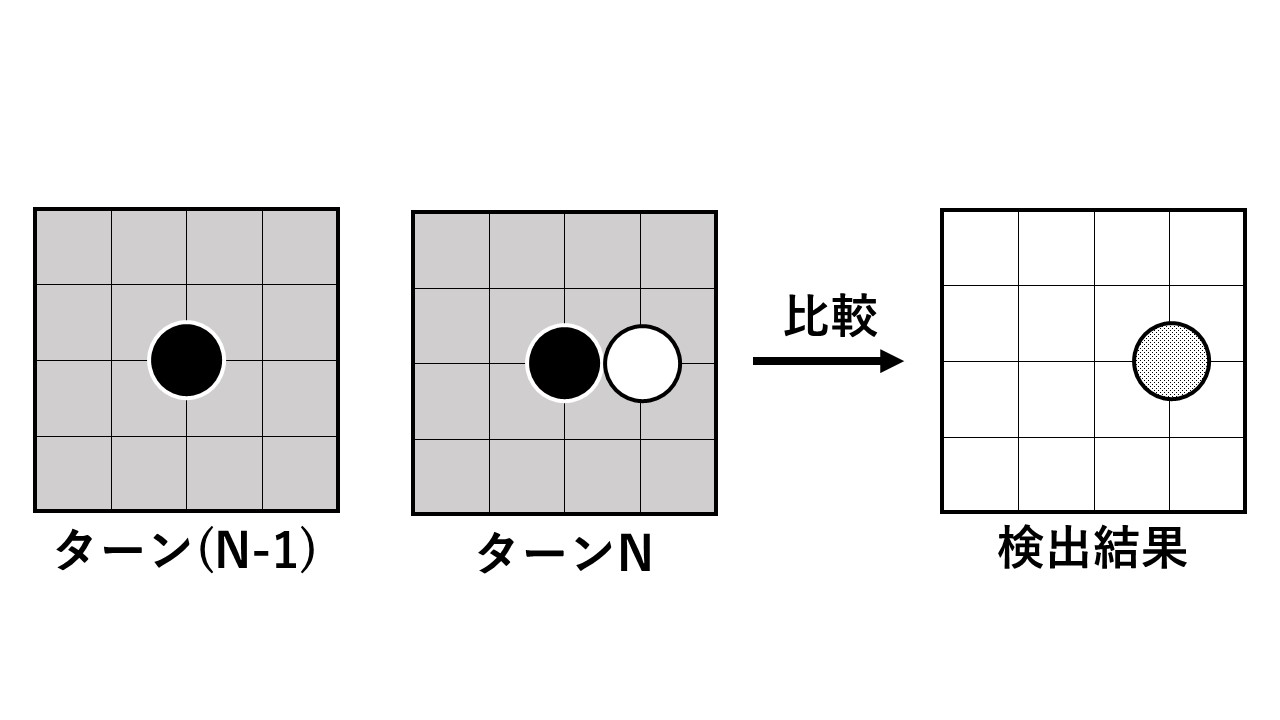
\includegraphics[clip,width=80mm]{PilotStudy_image.jpg} 
            \caption{先行研究の手法}
            \label{PS_img}
            \end{center}
        \end{figure}

            %TODO「なんでこの方法でやろうと思ったのか書けるといいね.」
        しかし,この手法では,途中から対局を記録しようとした時に,そのターンを記録できない問題が存在する.
        そこで本研究では,記録しようとした時点のターンから記録できるように,直前の着手の情報を使用せず,1つの着手の画像だけで碁石の位置を検出することを目的とする.
        また,先行研究の手法では,横320$\times$縦240画素のカメラが使用されており,碁石の識別は約1画素の輝度をもとに行われる.
        本研究では,より高解像度のカメラを使用し,一定の領域内に存在する全画素の輝度値をもとに碁石の種類の検出を行うことで精度向上を図る.

    \section{理論} % セクション.理論
    \label{config}
        \subsection{同次座標}
            座標$(x,y)$に対し,その要素を1つ増やした座標$(\xi_1,\xi_2,\xi_3)$を,以下の関係式を満たすように定義する.\\
            \begin{equation} % 同次座標の数式
                \begin{split} % 複数行に1つの式番号を与える
                    x = \frac{\xi_1}{\xi_3} \\ 
                    y = \frac{\xi_2}{\xi_3}
                \end{split}
                \label{Homogeneous}
            \end{equation}

            ただし,$\xi_1,\xi_2,\xi_3$のうち少なくとも1つは0ではないとする.このように定義される座標を同次座標と呼ぶ\cite{DIP}.

            同次座標においては$\lambda\neq0$なる任意の$\lambda$に対して,$(\xi_1,\xi_2,\xi_3)$と$(\lambda\xi_1,\lambda\xi_2,\lambda\xi_3)$は通常の座標に直したときともに$(\xi_1/\xi_3,\xi_2/\xi_3)$となるため,同じ点を表している.つまり,同次座標による表現では,定数倍をしても変わらないとみなすことができる.このような表現を同値であるとよび,これを式では以下のように表す.
            \begin{equation} % 同次座標の数式2
                \left(
                    \begin{array}{ccc}
                        \xi_1\\
                        \xi_2\\
                        \xi_3
                    \end{array}
                \right) \sim % \sim: 「~」
                \left(
                    \begin{array}{ccc}
                        \lambda\xi_1\\
                        \lambda\xi_2\\
                        \lambda\xi_3
                    \end{array}
                \right)
            \end{equation}
            ここで記号$\sim$は同値関係を表し,定数倍の違いを許して等しいことを意味する.

                %! http://www.info.hiroshima-cu.ac.jp/~miyazaki/knowledge/tech0115.html
        \subsection{射影変換}
            同次座標を利用することにより,一般的な変換を表現することができる.
            これは以下の式で表現されるもので,射影変換と呼ばれている\cite{DIP}.
            \begin{equation} % 射影変換の数式
                \left(
                    \begin{array}{ccc}
                    x'\\
                    y'\\
                    1
                    \end{array}
                \right)\sim
                \left(
                    \begin{array}{ccc}
                    h_{11} & h_{12} & h_{13}\\
                    h_{21} & h_{22} & h_{23}\\
                    h_{31} & h_{32} & h_{33}\\
                    \end{array}
                \right)
                \left(
                    \begin{array}{ccc}
                    x\\
                    y\\
                    1
                    \end{array}
                \right)
                \label{Homography}
            \end{equation}
            あるいは,これをベクトルと行列の記号を用いて,以下のように表現することもできる.
            \begin{equation} % 射影変換のベクトル数式
                \bm{\vec{x}'} \sim \bm{H\vec{x}}
            \end{equation}
            $\bm{H}$は任意の$3\times3$の行列である.これを変換行列という.

            式(\ref{Homogeneous})の関係を用いて,(\ref{Homography})から座標$(x',y')$を求めると以下のように表すことができる.
            \begin{equation} % 変換行列を用いてx,yを表現する式
                \begin{split} % 複数行に1つの式番号を与える
                    x' = \frac{h_{11}x+h_{12}y+h_{13}}{h_{31}x+h_{32}y+h_{33}} \\ 
                    y' = \frac{h_{21}x+h_{22}y+h_{23}}{h_{31}x+h_{32}y+h_{33}} \\ 
                \end{split}
                \label{transform_XY}
            \end{equation}

            一意に射影変換の変換行列を表すため,行列のどれか1つの値を固定する.$h_{33}=1$とし,(\ref{transform_XY})に代入,式変形を行うと$(x',y')$は以下のように表すことができる.
            \begin{equation} % 変換行列を用いてx,yを表現する式
                \begin{split} % 複数行に1つの式番号を与える
                    xh_{11}+yh_{12}+h_{13}-xx'h_{31}-yx'h_{32} = x'\\ 
                    xh_{21}+yh_{22}+h_{23}-xy'h_{31}-yy'h_{32} = x'\\ 
                \end{split}
                \label{transform_XY_ALT}
            \end{equation}

            (\ref{transform_XY_ALT})をベクトル演算で表記すると,以下のように表記できる.
            \footnotesize
            \begin{equation}
                \begin{split}
                    (x,y,1,0,0,0,-xx',-yx') (h_{11},h_{12},\cdots,h_{31},h_{32})^T \\
                    (0,0,0,x,y,1,-xy',-yy') (h_{11},h_{12},\cdots,h_{31},h_{32})^T
                \end{split}
                \label{transform_XY_Vector}
            \end{equation}
            \normalsize

            2つの四角形の頂点座標をそれぞれ
            $((x_{11},y_{11}),(x_{12},y_{12}),(x_{13},y_{13}),(x_{14},y_{14}))$,$((x_{21},y_{21}),(x_{22},y_{22}),(x_{23},y_{23}),(x_{24},y_{24}))$
            とすると,すべての頂点を(\ref{transform_XY_Vector})で表すと以下の式になる.
            \fontsize{7.5pt}{0pt}
            \begin{equation} % 8*8
                \left(
                \begin{matrix}
                    x_{11},y_{11},1,0,0,0,-x_{11}x_{21},-y_{11}x_{21}\\
                    0,0,0,x_{11},y_{11},1,-x_{11}y_{21},-y_{11}y_{21}\\
                    x_{12},y_{12},1,0,0,0,-x_{12}x_{22},-y_{12}x_{22}\\
                    0,0,0,x_{12},y_{12},1,-x_{12}y_{22},-y_{12}y_{22}\\
                    x_{13},y_{13},1,0,0,0,-x_{13}x_{23},-y_{13}x_{23}\\
                    0,0,0,x_{13},y_{13},1,-x_{13}y_{23},-y_{13}y_{23}\\
                    x_{14},y_{14},1,0,0,0,-x_{14}x_{24},-y_{14}x_{24}\\
                    0,0,0,x_{14},y_{14},1,-x_{14}y_{24},-y_{14}y_{24}\\
                \end{matrix}
                \right)
                \left(
                \begin{matrix}
                    h_{11}\\
                    h_{12}\\
                    h_{13}\\
                    h_{21}\\
                    h_{22}\\
                    h_{23}\\
                    h_{31}\\
                    h_{32}\\
                \end{matrix}
                \right)
                =
                \left(
                \begin{matrix}
                    x_{21}\\
                    y_{21}\\
                    x_{22}\\
                    y_{22}\\
                    x_{23}\\
                    y_{23}\\
                    x_{24}\\
                    y_{24}\\
                \end{matrix}
                \right)
                \label{8x8vector}
            \end{equation}
            \normalsize
            よって,(\ref{8x8vector})の左辺にある$8\times8$行列の逆行列を計算することで,射影変換の変換行列の各要素が求まる\cite{SquareTransform}.
            \fontsize{6.5pt}{0pt}
            \begin{equation} % 8*8
                \left(
                    \begin{matrix}
                        h_{11}\\
                        h_{12}\\
                        h_{13}\\
                        h_{21}\\
                        h_{22}\\
                        h_{23}\\
                        h_{31}\\
                        h_{32}\\
                    \end{matrix}
                    \right)
                    =    
                \left(
                \begin{matrix}
                    x_{11},y_{11},1,0,0,0,-x_{11}x_{21},-y_{11}x_{21}\\
                    0,0,0,x_{11},y_{11},1,-x_{11}y_{21},-y_{11}y_{21}\\
                    x_{12},y_{12},1,0,0,0,-x_{12}x_{22},-y_{12}x_{22}\\
                    0,0,0,x_{12},y_{12},1,-x_{12}y_{22},-y_{12}y_{22}\\
                    x_{13},y_{13},1,0,0,0,-x_{13}x_{23},-y_{13}x_{23}\\
                    0,0,0,x_{13},y_{13},1,-x_{13}y_{23},-y_{13}y_{23}\\
                    x_{14},y_{14},1,0,0,0,-x_{14}x_{24},-y_{14}x_{24}\\
                    0,0,0,x_{14},y_{14},1,-x_{14}y_{24},-y_{14}y_{24}\\
                \end{matrix}
                \right)^{-1}
                \left(
                \begin{matrix}
                    x_{21}\\
                    y_{21}\\
                    x_{22}\\
                    y_{22}\\
                    x_{23}\\
                    y_{23}\\
                    x_{24}\\
                    y_{24}\\
                \end{matrix}
                \right)      
                \label{8x8vector_Inverse}
            \end{equation}
            \normalsize

            射影変換においては,線分の直線性は保たれるものの,平行性は失われる.別の言い方をすると,任意の四角形を別の任意の四角形に移すような変換であるといえる.

            射影変換の模式図を図\ref{sample_homography}に示す.

            \begin{figure}[tb] % 射影変換の模式図
                \begin{center}
                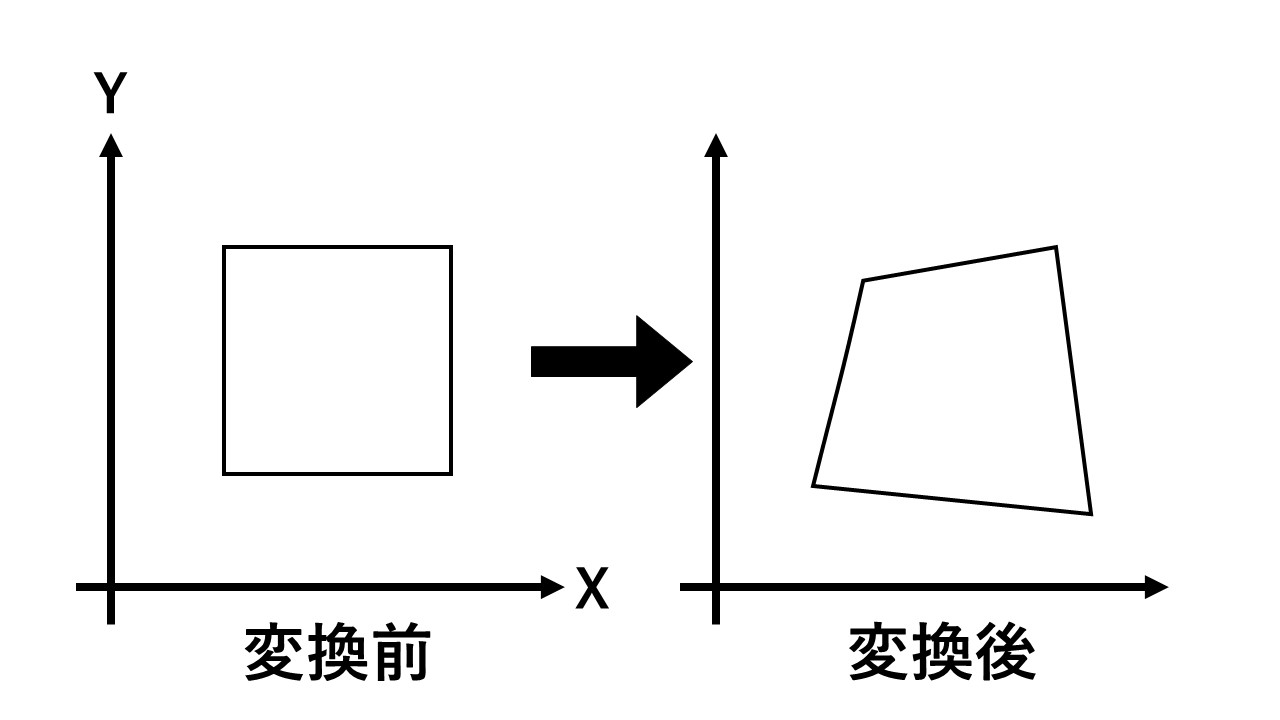
\includegraphics[clip,width=90mm]{Homography.jpg} 
                \caption{射影変換の模式図}
                \label{sample_homography}
                \end{center}
            \end{figure}
    

        % 2.2
        %TODO 教科書の図っぽいのを作って挿入とか,フィルタの論文について言及するとか.
        \subsection{空間フィルタ}
            入力画像の対応する画素値だけでなく,その周囲の画素も含めた領域内の画素値を用いて計算する処理のことを空間フィルタリングといい,この処理で用いるフィルタを空間フィルタという\cite{DIP}.
            
            空間フィルタは,線形フィルタと非線形フィルタの2つに分類できる.

            線形フィルタは,入力画像を$f(i,j)$,出力画像を$g(i,j)$とするとき,以下の式で表すことができるフィルタのことをいう.
            \begin{equation} \label{linear_filter}
                g(i,j) = \sum\limits_{n=-W}^{W}\sum\limits_{m=-W}^{W}f(i+m,j+n)h(m,n)
            \end{equation}
            $h(m,n)$はフィルタの係数を表す配列であり,フィルタの大きさは$(2W+1)\times(2W+1)$である.

            非線形フィルタは,(\ref{linear_filter})式に当てはまらない処理を伴うフィルタである.

        \subsection{メディアンフィルタ}
            フィルタ範囲内のピクセルの画素値を昇順か降順に並び替え,中央値を出力するフィルタをメディアンフィルタと呼ぶ\cite{DIP}.
            これは非線形フィルタに属する.
            $3\times3$の画素に対しメディアンフィルタを適用した際の例を図\ref{medianBlur}に示す.

            \begin{figure}[tb] % メディアンフィルタの図
                \begin{center}
                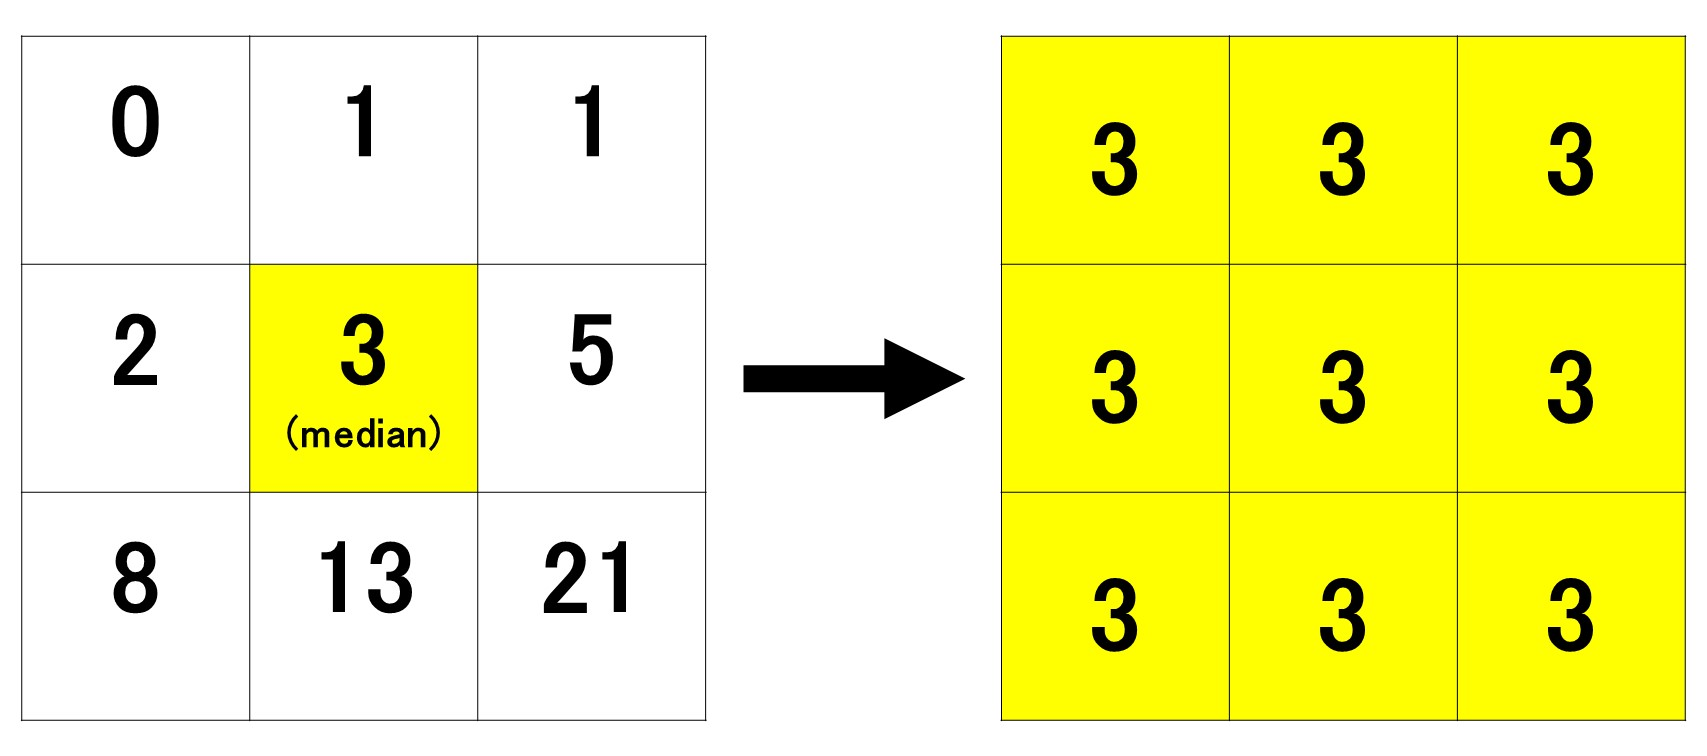
\includegraphics[clip,width=80mm]{medianBlur.jpg} 
                \caption{メディアンフィルタの例}
                \label{medianBlur}
                \end{center}
            \end{figure}

            このフィルタは,コントラストの差がある輪郭部分がぼやけにくい特徴を持つ.
            同じ画像に対して,領域内の画素値の平均を出力するフィルタ(平均化フィルタ)とメディアンフィルタを施した例を,それぞれ図\ref{sample_average}と図\ref{sample_median}に示す.
            \begin{figure}[tb] % 平均化フィルタ,メディアンフィルタの2枚
                \begin{center}
                  \begin{tabular}{c}
                    \begin{minipage}{0.5\hsize}
                      \begin{center}
                        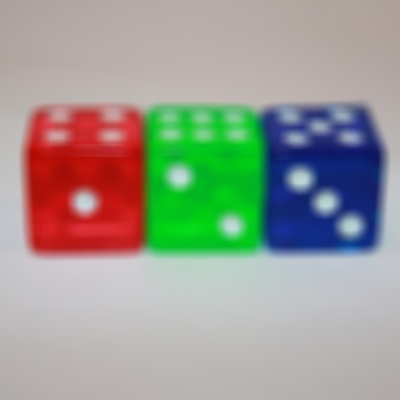
\includegraphics[clip,width=40mm]{sample_average.jpg}
                    \caption{平均化フィルタ}
                    \label{sample_average}
                      \end{center}
                    \end{minipage}
                    \begin{minipage}{0.5\hsize}
                      \begin{center}
                        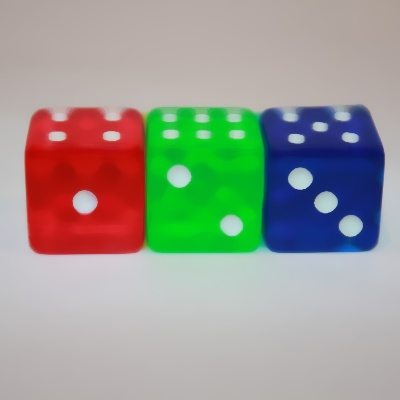
\includegraphics[clip,width=40mm]{sample_median.jpg}
                    \caption{メディアンフィルタ}
                    \label{sample_median}
                      \end{center}
                    \end{minipage}
                  \end{tabular}
                \end{center}
            \end{figure}

        \subsection{真陽性率・真陰性率} % 
            % https://jeaweb.jp/files/about_epi_research/contest2016_1_202007.pdf
            % https://bellcurve.jp/statistics/glossary/2014.html (こっちのほうが分かりやすいけど,参考文献には不適切な気がする.)
        検査で検出したい信号や疾患を有するもののうち,検査が正しく陽性と判断したものの割合のことを真陽性率(TPF: True Positive Fraction)と呼ぶ.
        この割合が大きいと,検出したい信号を有する対象に対して行った検査が誤って陰性と判断した割合(偽陰性率,FNF)は小さくなる.
        TPFとFNFの関係を以下に示す.
        \begin{align}
            TPF = 1-FNF
        \end{align}
        本研究では,白色(黒色)の碁石がある座標を,システムが「白石(黒石)がある」と識別した割合を指す.

        また,検査で検出したい信号や疾患を有さないもののうち,検査が正しく陰性と判断したものの割合を真陰性率(TNF: True Negative Fraction)と呼ぶ.
        この割合が大きいと,検出したい信号を有さない対象に対して行った検査が誤って陽性と判断した割合(偽陽性率,FPF)は小さくなる.
        TNFとFPFの関係を以下に示す.
        \begin{align}
            TNF = 1-FPF
        \end{align}
        本研究では,白色(黒色)の碁石がない座標を,システムが「白石(黒石)がない」と識別した割合を指す.

    \section{碁石識別システム} % セクション.システムについて
    \label{system}
            %TODO この章はもっと書けると思うので,全体的に説明を拡充しましょう!
                %! 目標は,後で他の人が同じ実験をできるように説明する,です
        本研究で検討したシステムでは,盤面を含む画像から,碁石の位置を識別することを目的とする.

        実際には,盤面を含む画像から盤面を切り抜き,碁石上の線を黒石と誤検知しないようノイズ処理を施した後に$19\times19$の領域を付与する.
        その後,付与した領域内における輝度値の平均を計算し,黒石・白石のしきい値とを比較,結果をもとに石の識別を行う.
        システムの流れを図\ref{flow}に示す.
        \begin{figure}[tb] % フロー図
            \begin{center}
            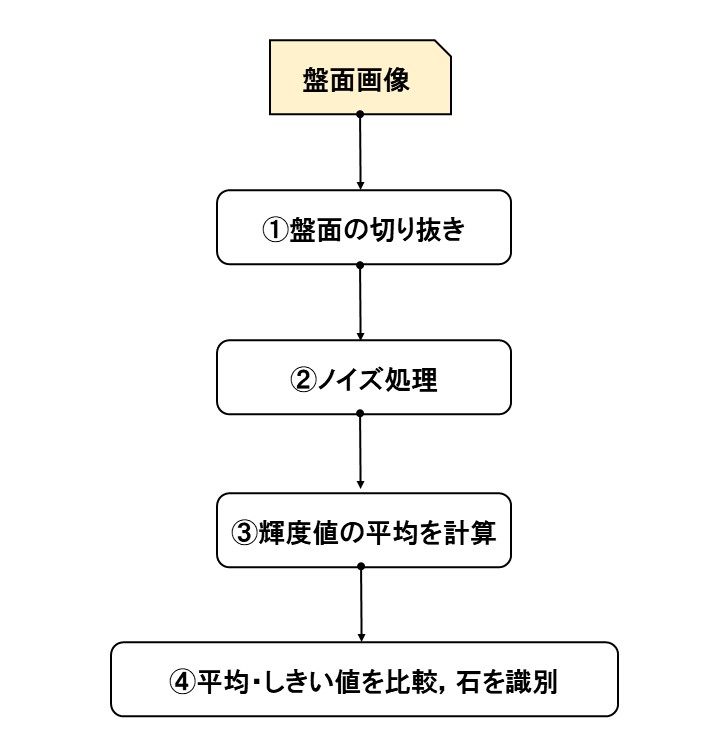
\includegraphics[clip,width=90mm]{flow.jpg} 
            \caption{フロー図}
            \label{flow}
            \end{center}
        \end{figure}

        %? ライブラリの比較,OpenCVを使った理由? 参考文献を探す
        システム中で行う処理には,プログラミング言語であるPythonと,オープンソースのコンピュータビジョン用ライブラリであるOpenCVを用いる.
        途中で行う射影変換の処理には,異なる画像処理ライブラリであるPillowやscikit-imageを用いても実装は可能であるが,複雑な計算を実装する必要がある.
        OpenCVであればこれを計算する関数が用意されており,処理を簡単に実装できるといった理由からOpenCVを選択した.

        \subsection{切り抜き}
        \label{boardCut}
            盤面を含む画像では,盤面以外の部分は不要である.
            そのため,盤面を含む画像から,盤面以外の不要な部分を除去する処理を行う.
            % 盤面画像の生成には,碁盤の頂点座標と,変換後の四角形の頂点座標を指定して変換行列を生成し,その行列を用いて射影変換を行う.

            OpenCVを用いた射影変換には,getPerspectiveTransform()関数と,warpPerspective()関数を用いる.処理の手順を以下に示す.

            はじめに,getPerspectiveTransform()関数に,第一引数には変換前の四角形の頂点座標リスト,第二引数には変換後の四角形の頂点座標リストを与えることで,変換行列の計算を行う.
            ここで,変換前の四角形の頂点座標リストとして,盤面の四隅の座標を格納したリストを与える.
            盤面部分を正方形に変換するため,変換後の四角形の頂点座標リストには,正方形の四隅の座標を格納したリストを与える.

            次に,warpPerspective()関数に,第一引数には画像情報を格納した変数,第二引数には求めた変換行列,第三引数には出力画像のサイズを与えることで,画像に対する射影変換を行う.

            今回の実験では,変換行列の計算に用いる変換後の正方形の頂点と,出力する画像のサイズに$800\times800$の正方形を与えた.
            変換前と変換後の画像を図\ref{cornerImg},図\ref{boardImg}に示す.

            \begin{figure}[tb] % 射影変換前の画像
                \begin{center}
                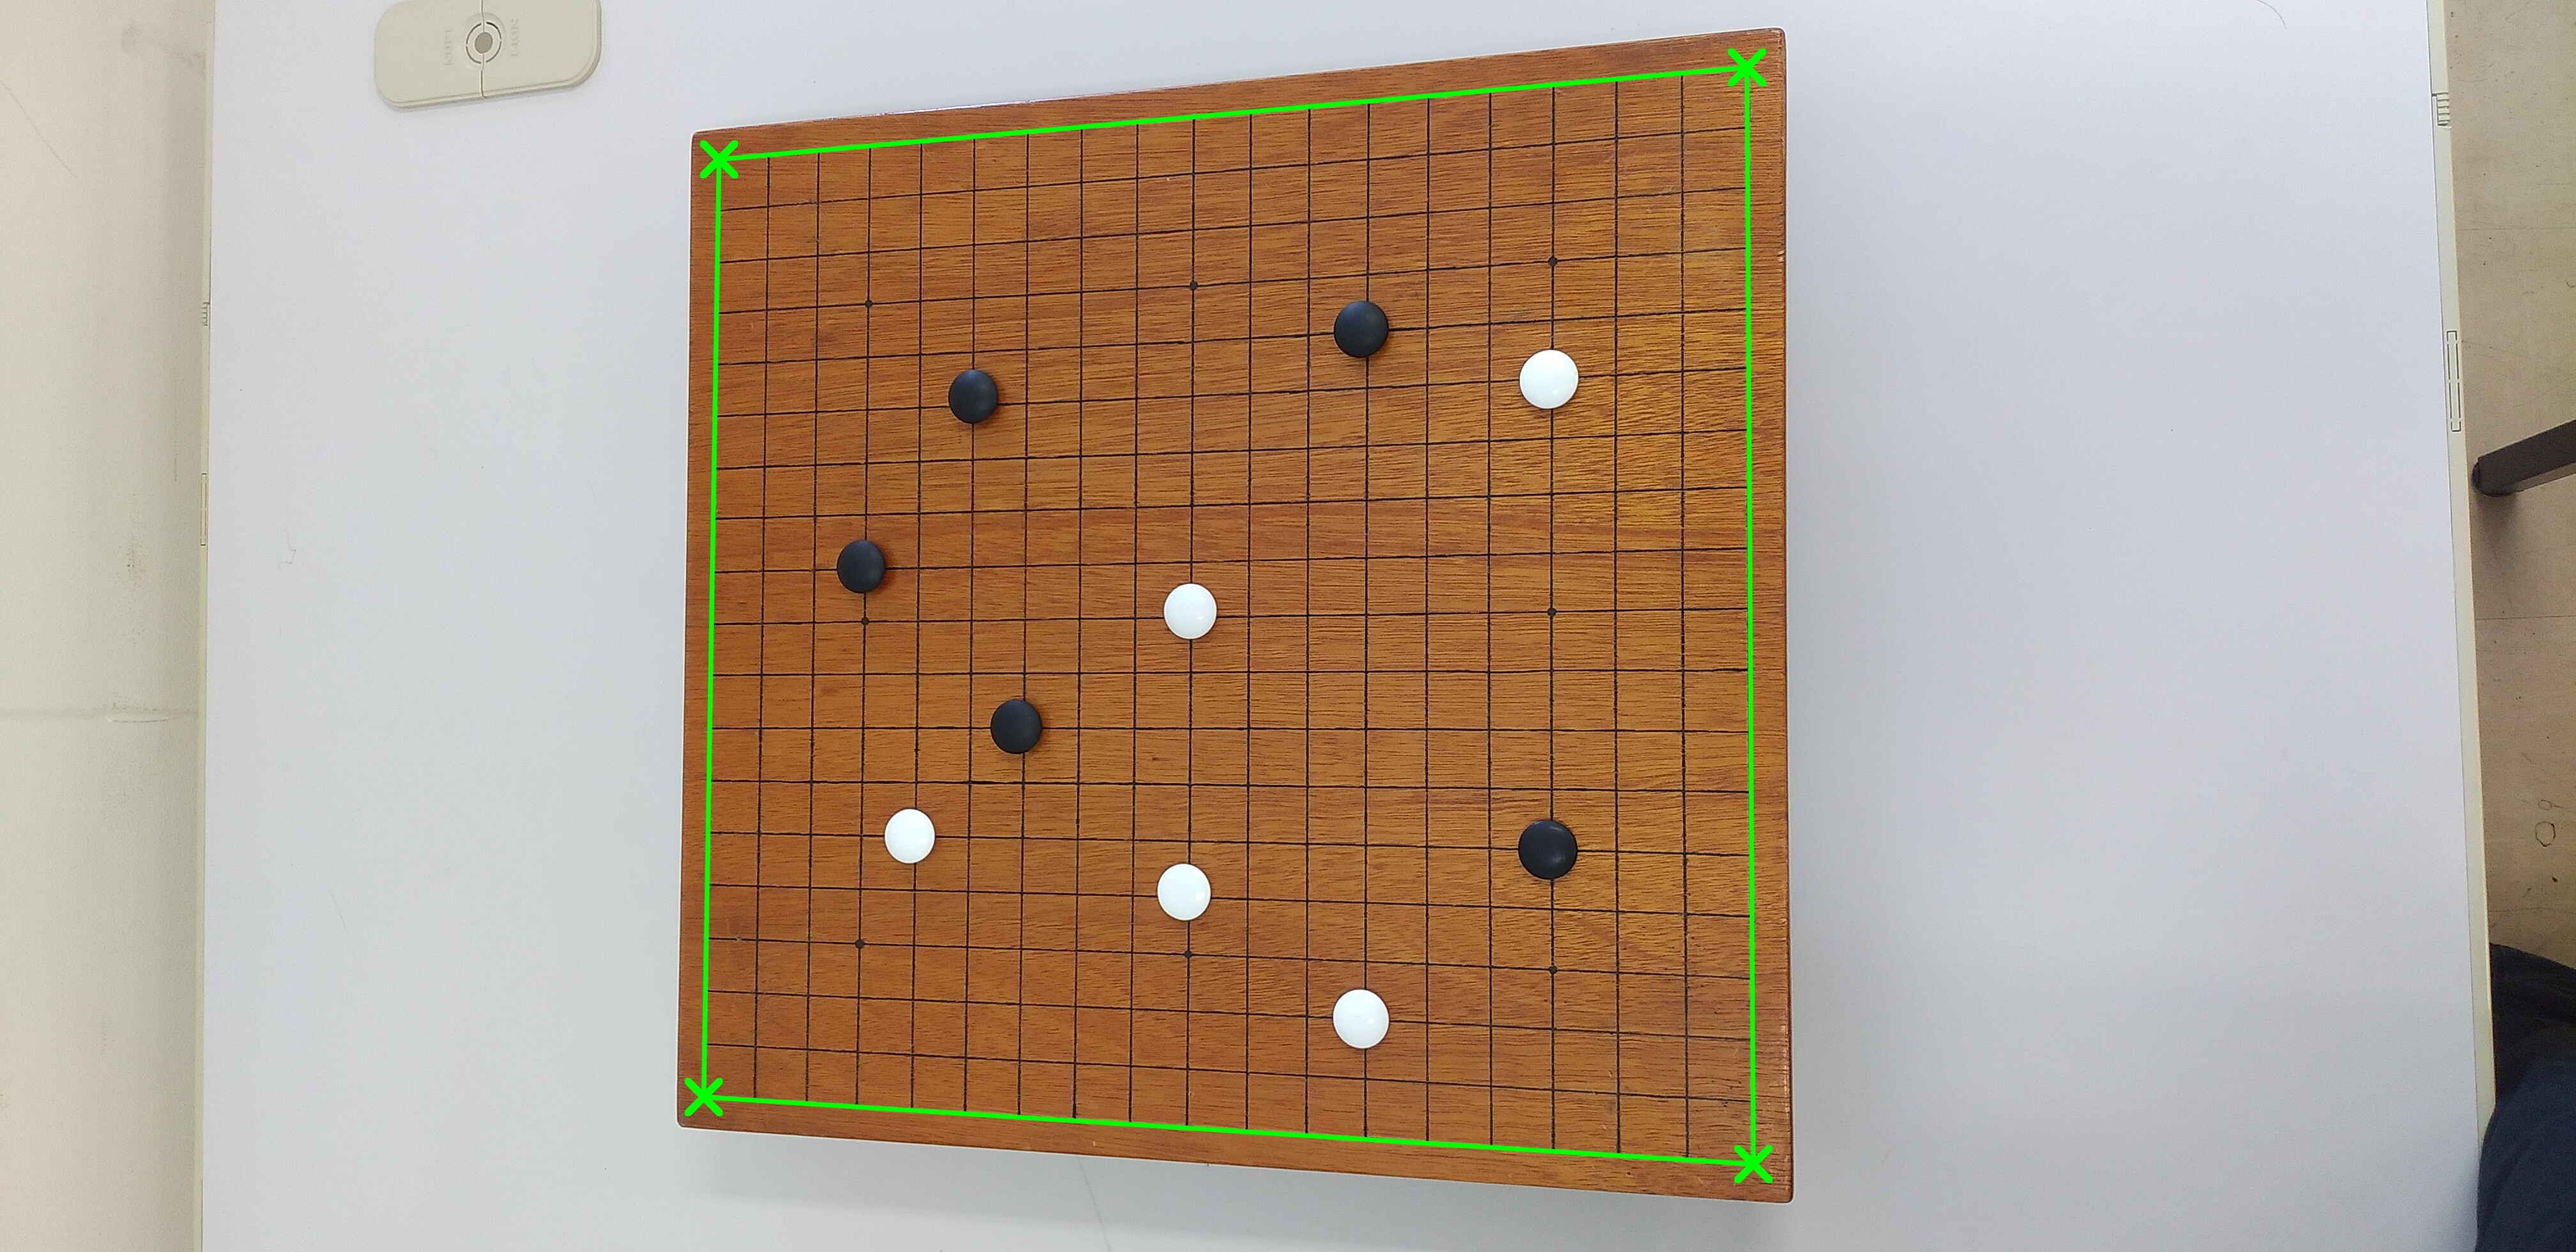
\includegraphics[clip,width=80mm]{DSC_0041/cornerImg.jpg} 
                \caption{射影変換前}
                \label{cornerImg}
                \end{center}
            \end{figure}
            \begin{figure}[tb] % 射影変換後の画像
                \begin{center}
                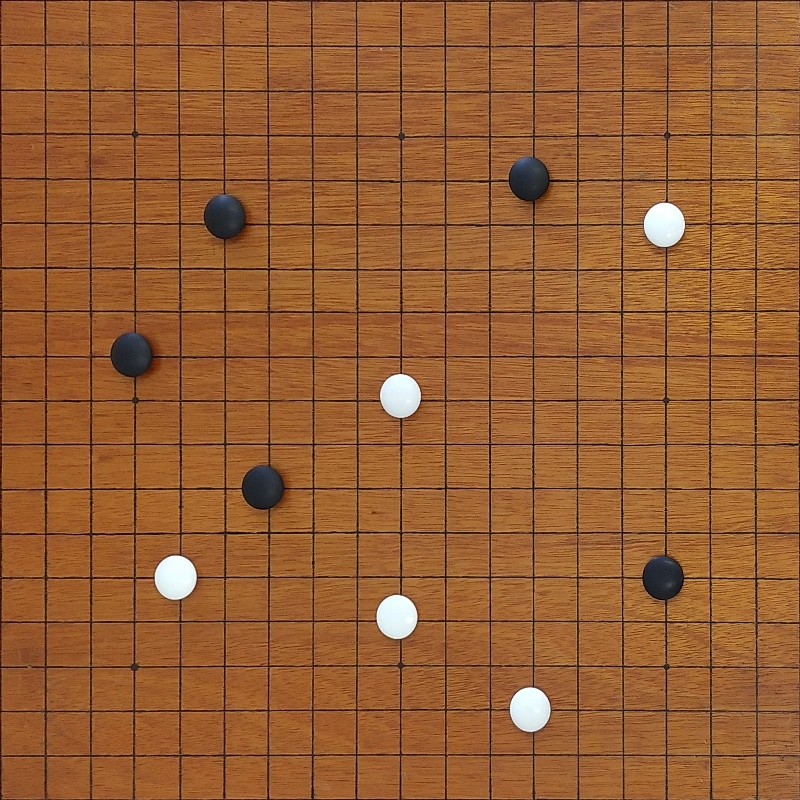
\includegraphics[clip,width=60mm]{DSC_0041/boardImg.jpg} 
                \caption{射影変換後}
                \label{boardImg}
                \end{center}
            \end{figure}

        %TODO グレースケール処理
        \subsection{グレースケール処理} \label{grayscale}
            白石と黒石の識別にはカラー画像でなくても行うことができると考える.
            そこで,本システムでは碁盤の画像に対しグレースケール処理を適用する.
            処理結果を図\ref{grayImg}に示す.
            \begin{figure}[tb] % 事例2,誤り部分・領域可視化版の2枚セット
                \begin{center}
                  \begin{tabular}{c}
                    \begin{minipage}{0.5\hsize}
                      \begin{center}
                        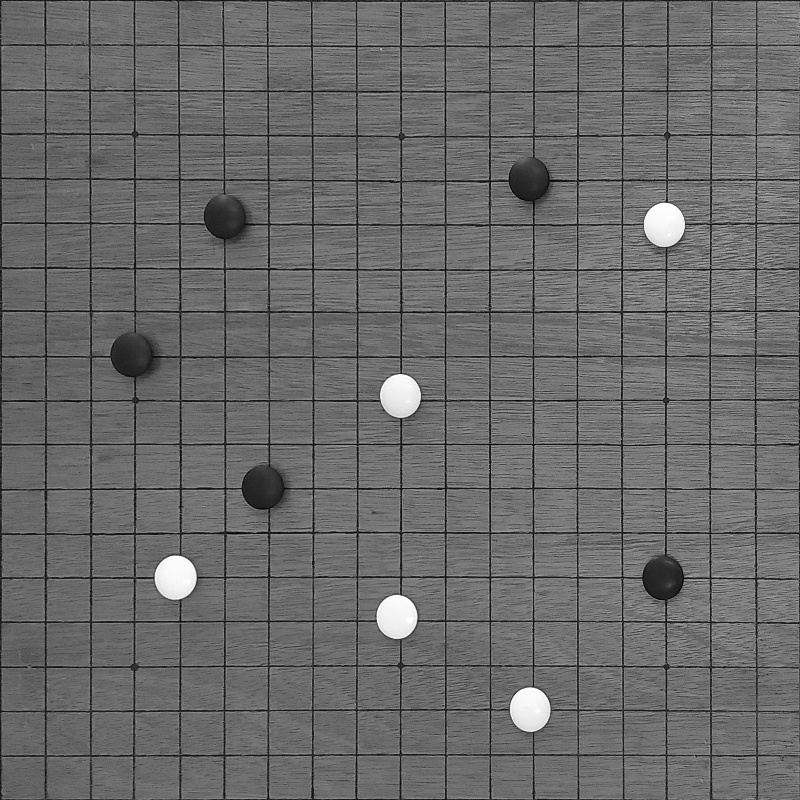
\includegraphics[clip,width=35mm]{DSC_0041/GRAYImg.jpg}
                    \caption{グレースケール処理}
                    \label{grayImg}
                      \end{center}
                    \end{minipage}
                    \begin{minipage}{0.5\hsize}
                      \begin{center}
                        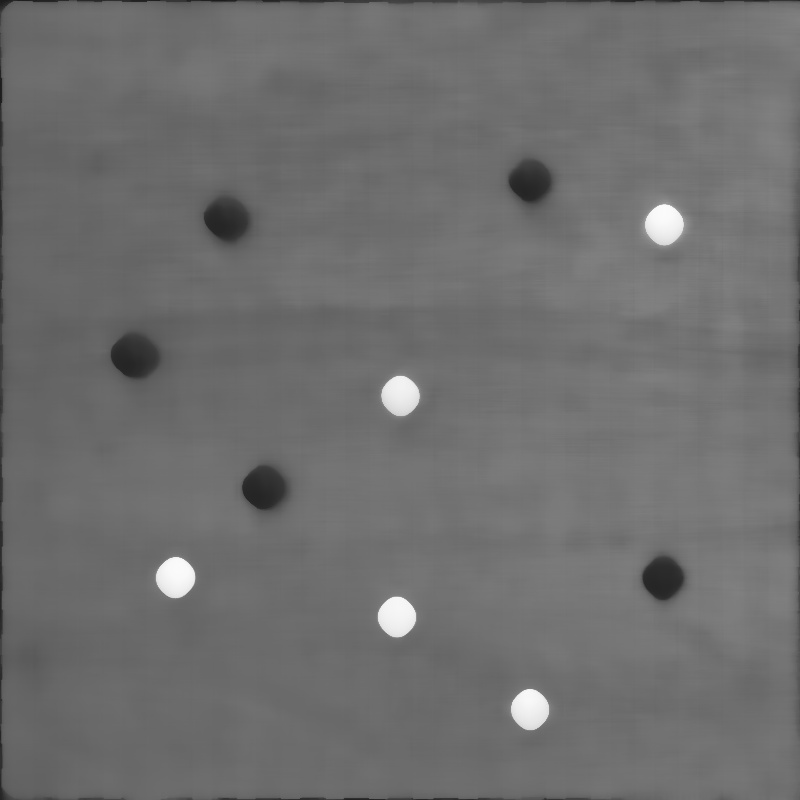
\includegraphics[clip,width=35mm]{DSC_0041/noiseReducedImg.jpg}
                    \caption{ノイズ除去後の盤面}
                    \label{noiseReducedImg}
                      \end{center}
                    \end{minipage}
                  \end{tabular}
                \end{center}
            \end{figure}


        \subsection{ノイズ除去} \label{noiseReduce}
            後述する識別の方法では,盤面上の線の交点を誤って黒石と識別してしまうことがある.
            これを減らすため,ノイズ処理を適用することで盤面上の線をある程度無視できるようにする. 
            \ref{grayscale}節で生成した画像(図\ref{grayImg})に対し,フィルタを用いてノイズ処理を行う.
            フィルタには,輪郭部分がぼやけにくいといった特徴を持つメディアンフィルタを使用する.
            なぜならば,メディアンフィルタは輪郭部分を残しやすいという特徴を持っているためである.
            たとえば平均値フィルタ(範囲内の画素値の平均を出力するフィルタ)は輪郭も曖昧にしてしまうという特徴がある.
            これに対し,メディアンフィルタは輪郭を残しやすいため,碁石の色が滲むことを防ぐことができる.
    
            OpenCVを用いたメディアンフィルタ処理は,medianBlur()関数に,第一引数に画像情報を格納した変数,第二引数にフィルタのカーネルサイズを与えることで実装できる.
            カーネルサイズの指定には奇数を用いる.
            これはメディアンフィルタの理論上,偶数のカーネルサイズを与えると中央値が求められないためである.
            今回の実験ではカーネルサイズに25を与えたことで,後に述べる識別で交点を誤って黒石と識別することを防ぐことができた.
            処理結果を図\ref{noiseReducedImg}に示す.

        \subsection{識別}
            \label{area}
            碁石の識別は,碁石が等間隔で設置されていることを利用して,盤面画像から等間隔で輝度値を取得することで実現できると考えた.% 過去形はどうなんだろう?
            識別の際に,輝度値の平均を取得するための$19\times19$個の小さな領域を付与する.
            \ref{noiseReduce}節で生成した図(図\ref{noiseReducedImg})に対し,各領域を緑色の四角形で表した画像を図\ref{boardWithArea}に示す.
            \begin{figure}[tb] % 領域を可視化した図
                \begin{center}
                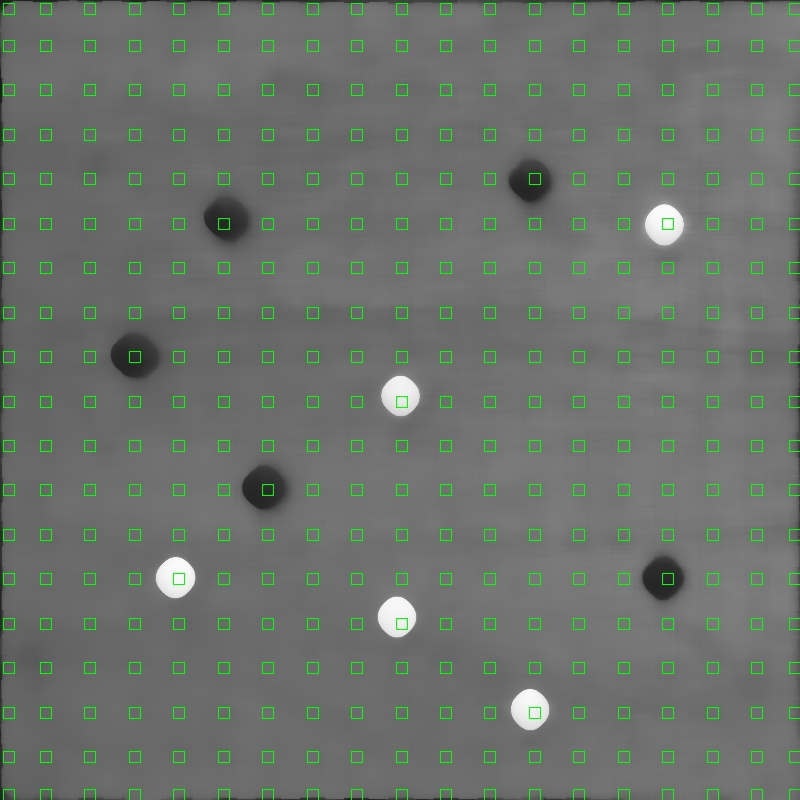
\includegraphics[clip,width=60mm]{DSC_0041/boardWithAreaImg.jpg} 
                \caption{領域を可視化した盤面}
                \label{boardWithArea}
                \end{center}
            \end{figure}

            与えた領域内における輝度値(0~255)の平均を取得し,白黒それぞれのしきい値をもとに各領域を
            \begin{itemize} % 3種類
                \item 平均値が黒石のしきい値より小さい = 「黒石がある」
                \item 平均値が白石のしきい値より大きい = 「白石がある」
                \item 「それ以外」
            \end{itemize}
            の3種類に分類することで,碁石の識別を行う.
            盤面のグレースケール画像(図\ref{grayImg})上に,実際に識別した結果を重ねた画像を図\ref{result}に示す.
            赤色の「$\times$」は黒石を識別した座標,青色の「$\times$」は白石を識別した座標,黄色の「$+$」はそれ以外の座標を意味する.

            \begin{figure}[tb] % 領域を可視化した図
                \begin{center}
                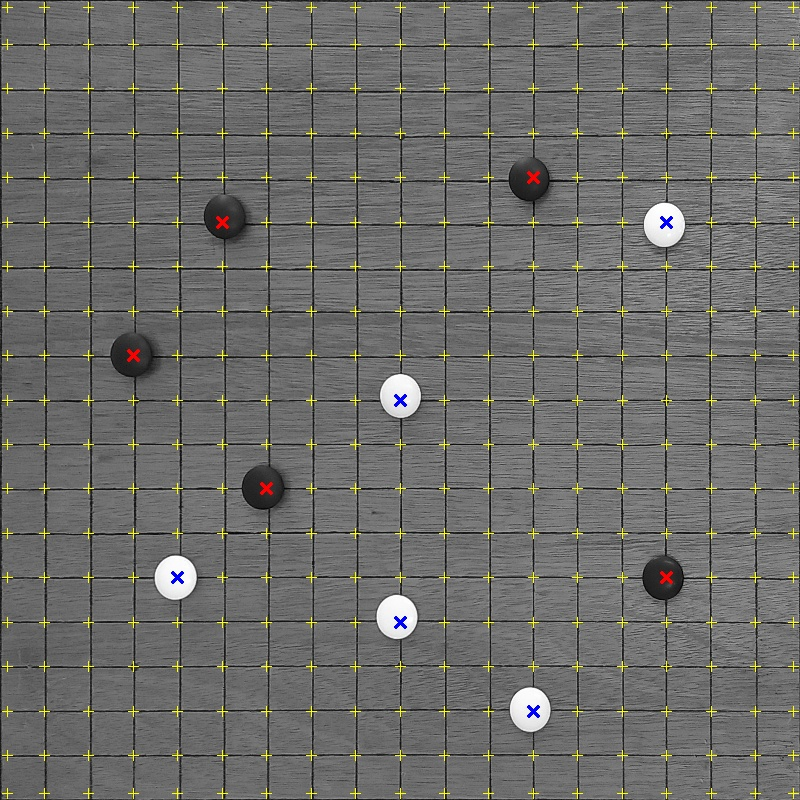
\includegraphics[clip,width=60mm]{DSC_0041/result.jpg} 
                \caption{識別結果を重ねた盤面}
                \label{result}
                \end{center}
            \end{figure}

    \section{実験と考察} % セクション.実験
            %TODO 実験の目的をこの章のどこかに書こう
                %? 研究の目的(碁石の位置認識)を実現するために,何を明らかにしようと思ってこの実験をやったんだっけ,というのを書いてほしいな.
                %? (逆に言うと,何を明らかにすれば碁石の位置認識を実現できた!と言える?)
        本章では\ref{system}章で検討したシステムの有効性を検証するため,実際に盤面を含む画像を使ってシステムを適用し結果を考察する.

        \ref{threshold}節では,最適なしきい値を決定するために行った予備実験について示す.
        \ref{identify_result}節では,決定したしきい値のもとで,複数の事例に対し実際にシステムで碁石の識別を行った結果について示す.

        \subsection{予備実験} \label{threshold}
            どのしきい値で最も正確に識別を行えるか確認するために,2枚の盤面画像(図\ref{DSC0087},図\ref{DSC0100})に対しシステムを適用して碁石の識別を行う.
            しきい値を変化させながらシステムを適用し,しきい値の変動に対応して変動した以下の4項目によって,最適な値を決定する.
            \begin{itemize}
                \item 白石を,白石と識別した割合(白石の真陽性率)
                \item 黒石を,黒石と識別した割合(黒石の真陽性率)
                \item 白石でないものを,正しく白石でないと識別した割合(白石の真陰性率)
                \item 黒石でないものを,正しく黒石でないと識別した割合(黒石の真陰性率)
            \end{itemize}

            図\ref{DSC0087},図\ref{DSC0100}におけるしきい値を横軸に,縦軸には白石の真陽性率と真陰性率の割合をプロットしたグラフをそれぞれ図\ref{Case1White}と図\ref{Case2White}に,
            縦軸に黒石の真陽性率と真陰性率をプロットしたグラフをそれぞれ図\ref{Case1Black}と図\ref{Case2Black}に示す.
            図\ref{Case1White},図\ref{Case2White}より,図\ref{DSC0087}と図\ref{DSC0100}の両方に対し白石のしきい値は156~160の範囲で真陽性率100\%,真陰性率100\%を記録したため,以降の実験ではその範囲の中央値である158を使用する.
            また図\ref{Case1Black}と図\ref{Case2Black}より,図\ref{DSC0087}と図\ref{DSC0100}の両方に対し黒石のしきい値は52で真陽性率100\%,真陰性率100\%を記録したため,以降の実験では52を使用する.

            \begin{figure}[tb] % DSC_0087
                \begin{center}
                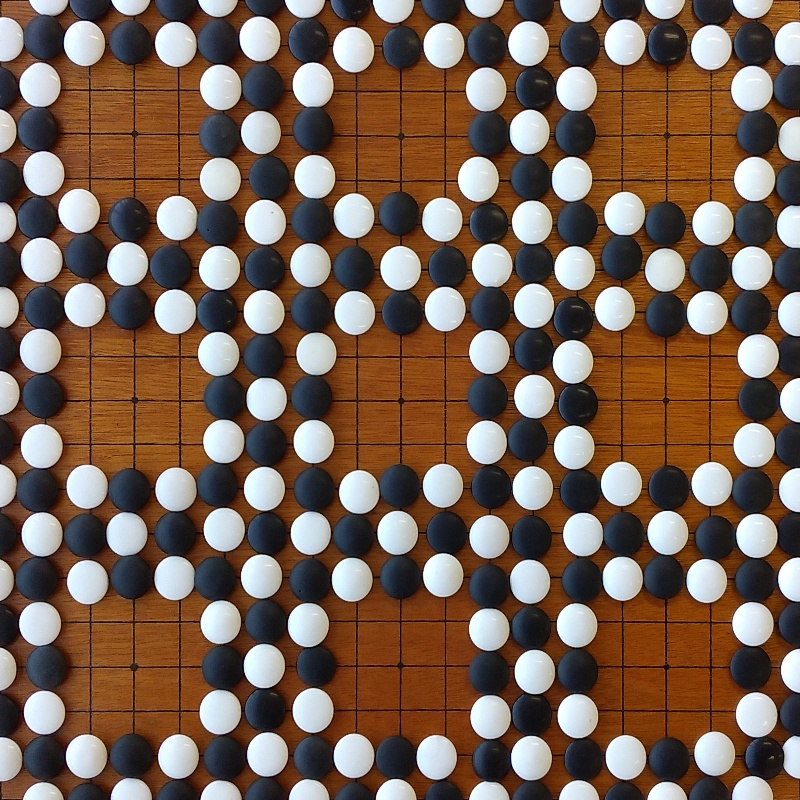
\includegraphics[clip,width=60mm]{DSC_0087/boardImg.jpg} 
                \caption{しきい値の決定に用いた盤面1}
                \label{DSC0087}
                \end{center}
            \end{figure}

            \begin{figure}[tb] % DSC_0100
                \begin{center}
                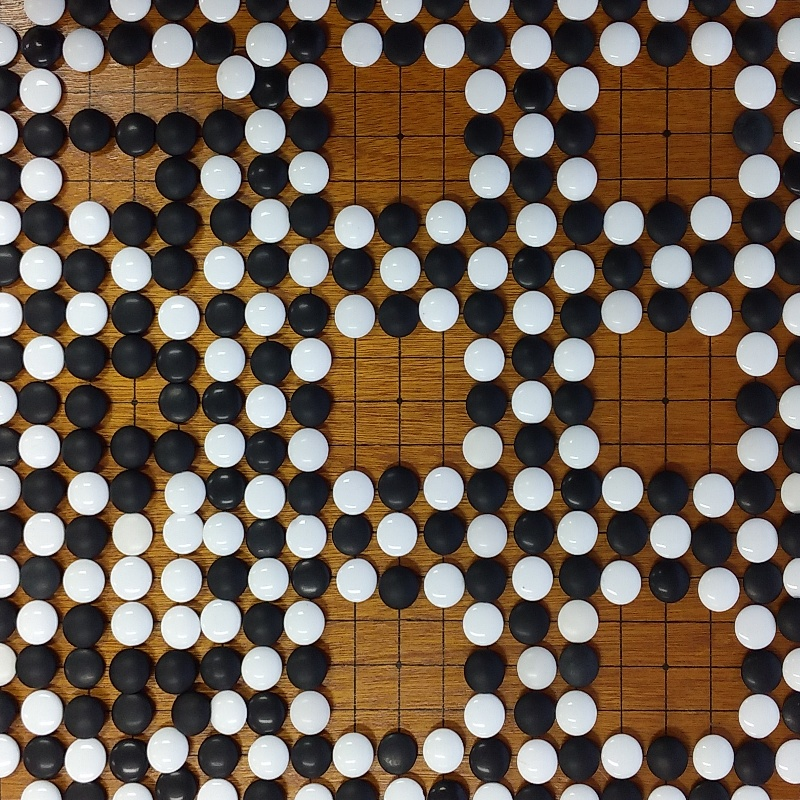
\includegraphics[clip,width=60mm]{DSC_0100/boardImg.jpg} 
                \caption{しきい値の決定に用いた盤面2}
                \label{DSC0100}
                \end{center}
            \end{figure}

            \begin{figure}[tb] % 白石の真陽性率・真陰性率1
                \begin{center}
                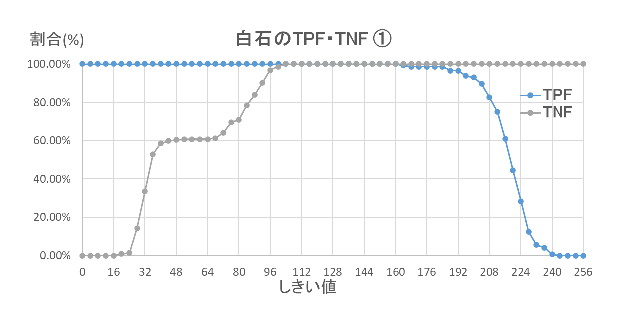
\includegraphics[clip,width=80mm]{Case1_White_TPF_TNF.eps} 
                \caption{白石の真陽性率・真陰性率1}
                \label{Case1White}
                \end{center}
            \end{figure}
            
            \begin{figure}[tb] % 白石の真陽性率・真陰性率2
                \begin{center}
                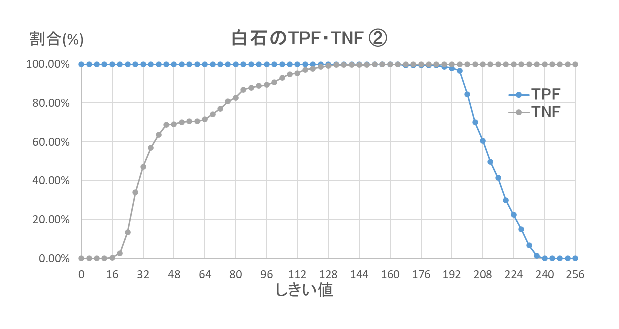
\includegraphics[clip,width=80mm]{Case2_White_TPF_TNF.eps} 
                \caption{白石の真陽性率・真陰性率2}
                \label{Case2White}
                \end{center}
            \end{figure}

            \begin{figure}[tb] % 黒石の真陽性率・真陰性率1
                \begin{center}
                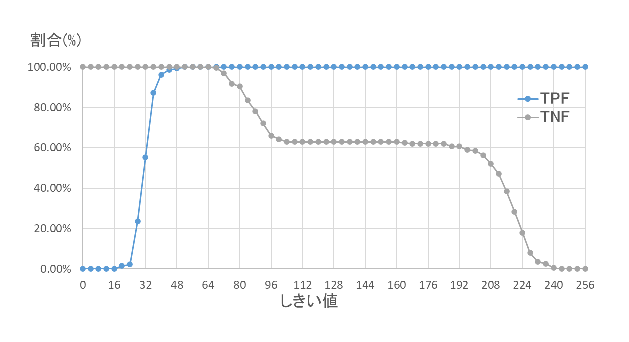
\includegraphics[clip,width=80mm]{Case1_Black_TPF_TNF.eps} 
                \caption{黒石の真陽性率・真陰性率1}
                \label{Case1Black}
                \end{center}
            \end{figure}

            \begin{figure}[tb] % 黒石の真陽性率・真陰性率2
                \begin{center}
                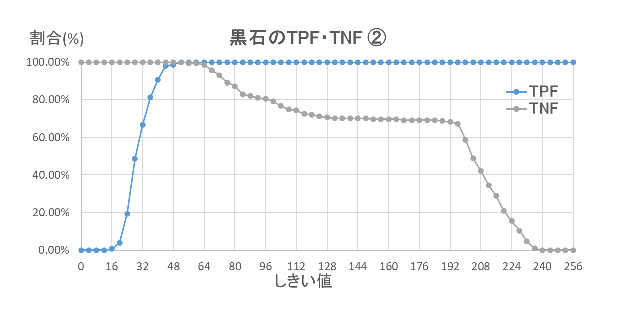
\includegraphics[clip,width=80mm]{Case2_Black_TPF_TNF.eps} 
                \caption{黒石の真陽性率・真陰性率2}
                \label{Case2Black}
                \end{center}
            \end{figure}

        \subsection{実際の識別結果} % 完全な成功例.DSC_0041
        \label{identify_result}
            本節では,3件の画像に対してシステムを適用した結果と,その考察を述べる.
            %? この下の文,冗長な気がする
            具体的には,すべて正常に識別できた場合,石の位置がずれていることで誤った識別をした場合,反射光を白石と誤った場合の識別結果について述べる.

            識別に用いた3つの盤面画像は,スマートフォンで撮影した$4032\times1960$pxの画像に対し,射影変換を用いて盤面を切り出した$800\times800$pxの画像である.

            \subsubsection{事例1}
                石の位置にずれがなく反射光の映り込みが少ない状況に対し,システムを適用する.

                この盤面画像(図\ref{ex1})に対しシステムを適用した結果,全ての碁石を正確に識別できた.
                図\ref{ex1}に対し,識別結果のマークを重ねた画像を図\ref{ex1_result}に示す.
                \begin{figure}[tb] % 事例1_盤面
                    \begin{center}
                    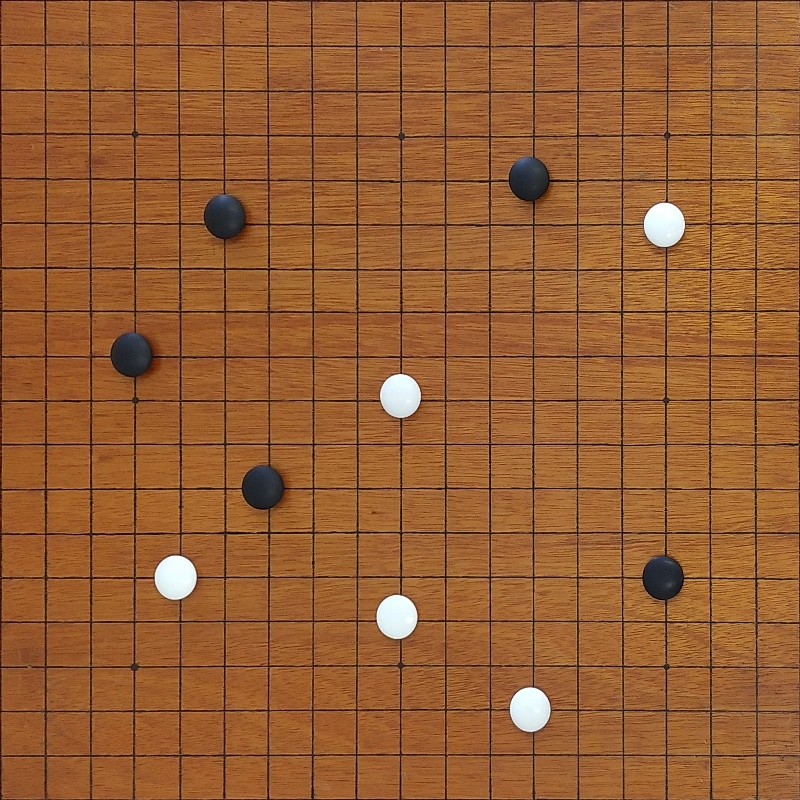
\includegraphics[clip,width=60mm]{DSC_0041/boardImg.jpg} 
                    \caption{事例1の盤面}
                    \label{ex1}
                    \end{center}
                \end{figure}

                \begin{figure}[tb] % 事例1_盤面結果
                    \begin{center}
                    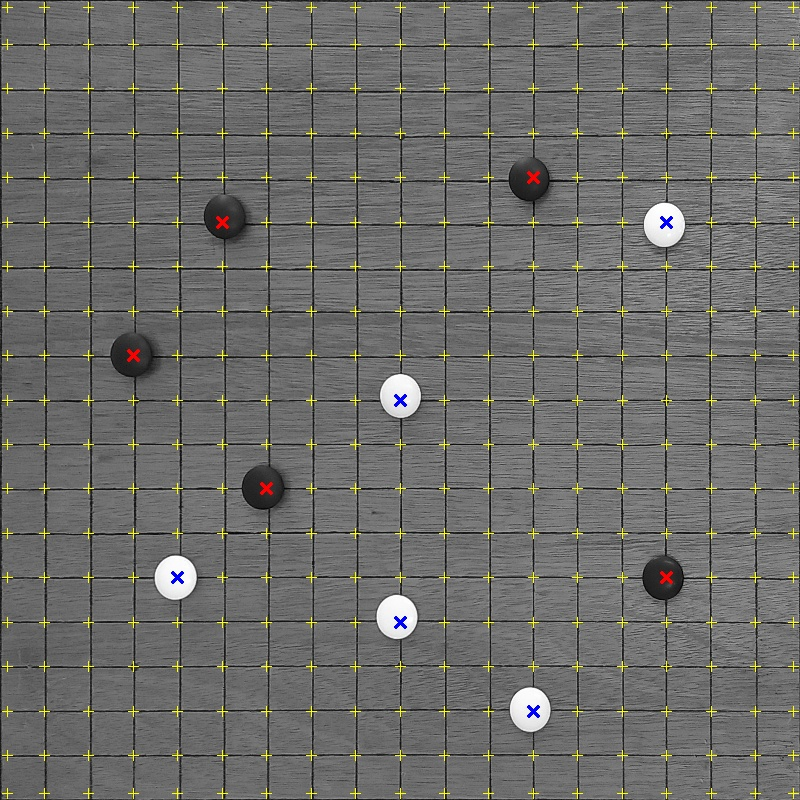
\includegraphics[clip,width=60mm]{DSC_0041/result.jpg} 
                    \caption{事例1の識別結果}
                    \label{ex1_result}
                    \end{center}
                \end{figure}

            \subsubsection{事例2} % 位置ズレによる失敗.DSC_0099.
                石の配置にずれがある状況に対しシステムを適用する.

                この盤面画像(図\ref{ex2_img})に対しシステムを適用した.
                実際は白石が置かれてあり,システムが「石がない」と誤って識別した位置の周囲を緑色の四角形で示す.
                緑の四角形で囲んだ範囲を拡大し,誤って識別した位置に記号を付与した画像を図\ref{ex2_error}に示す.

                図\ref{ex2_error}の範囲に対し,図\ref{noiseReducedImg}と同様に,輝度値の平均を取得する領域を可視化した画像を図\ref{ex2_error_area}に示す.
                図の中央部分を見ると,碁石の大部分が領域からはみ出ているのが分かる.
                このことから,石が正しく盤面の交点上に配置されていない場合,システムは正常に石を識別できないと考える.
                %! これをどうすれば解決できるのか書く
                
                
                \begin{figure}[tb] % 事例2_盤面
                    \begin{center}
                    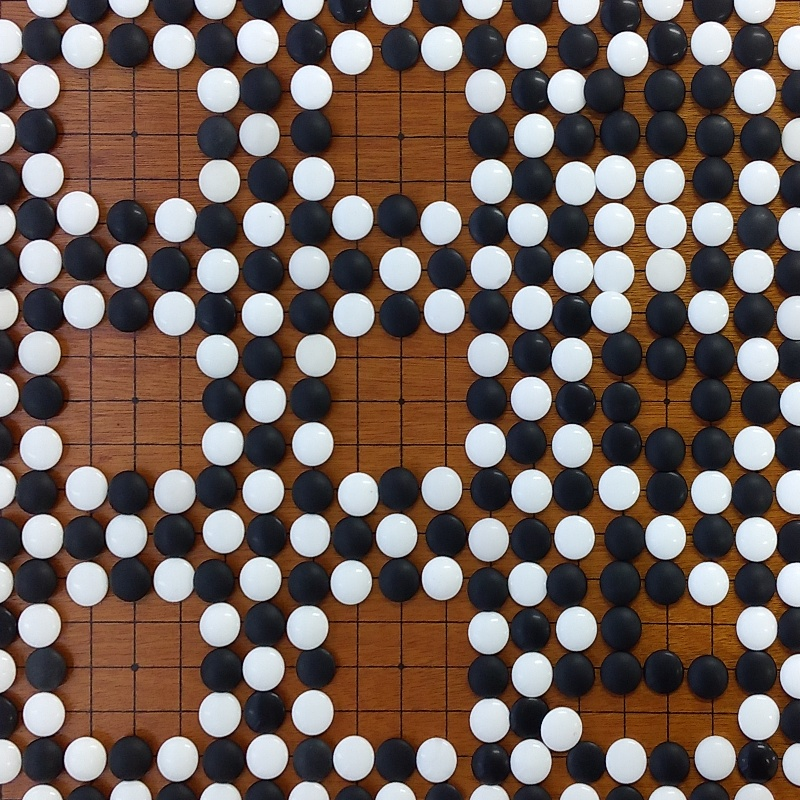
\includegraphics[clip,width=60mm]{DSC_0099/boardImg.jpg} 
                    \caption{事例2の盤面}
                    \label{ex2_img}
                    \end{center}
                \end{figure}

                \begin{figure}[tb] % 事例2,誤り部分・領域可視化版の2枚セット
                    \begin{center}
                      \begin{tabular}{c}
                        \begin{minipage}{0.5\hsize}
                          \begin{center}
                            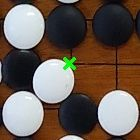
\includegraphics[clip,width=30mm]{DSC_0099/resultCompare_trim.jpg}
                        \caption{図\ref{ex2_img}の誤り部分}
                        \label{ex2_error}
                          \end{center}
                        \end{minipage}
                        \begin{minipage}{0.5\hsize}
                          \begin{center}
                            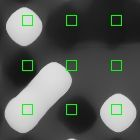
\includegraphics[clip,width=30mm]{DSC_0099/boardWithAreaImg_trim.jpg}
                        \caption{誤り部分の領域}
                        \label{ex2_error_area}
                          \end{center}
                        \end{minipage}
                      \end{tabular}
                    \end{center}
                \end{figure}
    
            \subsubsection{事例3} % 反射による失敗.DSC_0098.
                反射光が映り込んでいる状況に対しシステムを適用する.

                この盤面画像(図\ref{ex3_img})に対しシステムを適用した.
                実際は碁石が設置されておらず,システムが「白石がある」と誤って識別した位置の周囲を緑色の四角形で示す.
                緑の四角形で囲んだ範囲を拡大し,誤って識別した位置に記号を付与した画像を図\ref{ex3_error}に示す.

                図\ref{ex3_error}の範囲に対し,白石の識別に用いるしきい値よりも暗い部分を0,明るい部分を1として生成した二値画像を図\ref{ex3_error_area}に示す.
                これを見ると,白石が無い部分もしきい値以上の明るさであることが分かる.
                このことから,盤面や黒石に反射光が含まれているとシステムは誤って白石と識別すると考える.

                \begin{figure}[tb] % 事例3_盤面
                    \begin{center}
                    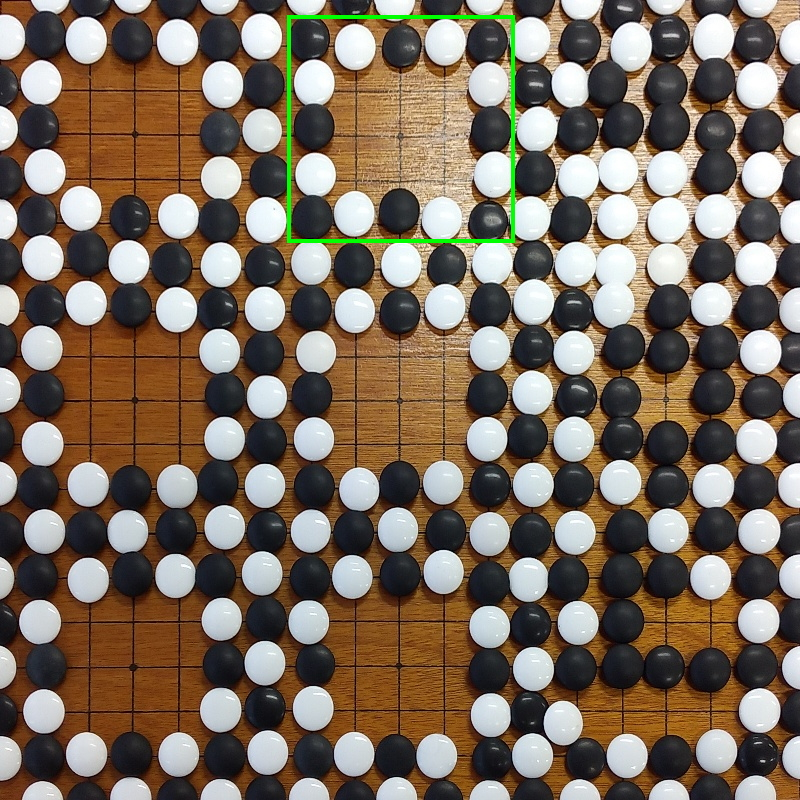
\includegraphics[clip,width=60mm]{DSC_0098/boardImg.jpg} 
                    \caption{事例3の盤面}
                    \label{ex3_img}
                    \end{center}
                \end{figure}

                \begin{figure}[tb] % 事例3,誤り部分,二値画像の2枚セット
                    \begin{center}
                      \begin{tabular}{c}
                        \begin{minipage}{0.5\hsize}
                          \begin{center}
                            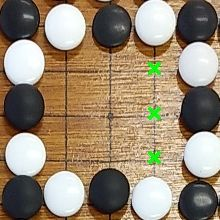
\includegraphics[clip,width=35mm]{DSC_0098/resultCompare_trim.jpg}
                        \caption{図\ref{ex3_img}の誤り部分}
                        \label{ex3_error}
                          \end{center}
                        \end{minipage}
                        \begin{minipage}{0.5\hsize}
                          \begin{center}
                            
\includegraphics[clip,width=35mm]{DSC_0098/inRange_WHITE_trim.jpg}
                        \caption{誤り部分の二値化}
                        \label{ex3_error_area}
                          \end{center}
                        \end{minipage}
                      \end{tabular}
                    \end{center}
                \end{figure}
                %! 反射光誤認の解決法を書く
                %TODO 反射光の誤認対策は?
                これは,白石と識別するしきい値を大きくすることで対策できると考える.
                実際にしきい値を158から190に設定することで,図\ref{ex3_error}の範囲の識別結果を改善することができた.
                しきい値を大きくした場合の,図\ref{ex3_error}と図\ref{ex3_error_area}と同じ範囲の識別結果を図\ref{ex3_alt}に示す.
                \begin{figure}[tb] % しきい値の拡大結果
                    \begin{center}
                    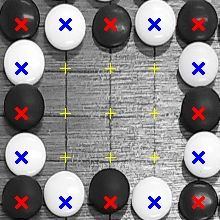
\includegraphics[clip,width=60mm]{DSC_0098/ALT_result_trim.jpg} 
                    \caption{しきい値を大きくした結果}
                    \label{ex3_alt}
                    \end{center}
                \end{figure}           
    
    \section{結言}\label{sec:Item} % 結言
        本研究では,囲碁の盤面を含んだ画像から碁石の配置を識別することを目的として,画像上から碁石の配置を識別するシステムの検討を行い,数件の画像に対してシステムを適用して有効性を確認した.

        \ref{identify_result}節より,本研究で検討したシステムでは石の位置に大きなずれが無い,かつ反射光が写り込んでいない場合に限り,碁石を正常に識別することができた.
        石のずれに対応できない問題には,画像に付与する領域(碁石座標)の位置を等間隔ではなく,碁盤の交点や石の形状をもとに検出することでこれを解決できると考える.
        反射光を誤って白石と識別する問題には,しきい値を固定するのではなく,画像の状況に応じて最適なしきい値を算出することや,画像上の反射光の写り込みを軽減させるノイズ処理で,誤った識別を減らすことができると考える.

        したがって,今後の課題として
        \begin{itemize}
            \item 石の座標を検出する手法
            \item 画像の状況に応じて適切なしきい値を算出する手法
            \item 反射光を軽減させるノイズ処理の手法
        \end{itemize}
        の模索が挙げられる.

    \section*{謝辞} %! 「*」を付けることで,セクションに章番号を付与しない
        本研究を進めるにあたり,様々なご指導を頂きました井上優良助教に深謝いたします.
        %先輩方のを見ると「研究室の同期」への謝辞だったけど,研究室だけじゃなくクラスメイト全体に感謝を示したい.こんな書き方でいいのか???
        また,この研究の機会をくださった情報工学科の先生方,そして多くの知識やご指摘を下さいました同級生の皆様に厚く御礼申し上げます.
    
    \begin{thebibliography}{10} % 参考文献

        % Webサイトの参考文献の書き方が怪しい.確認を取ること!

            % 書き方に困ったやつ.そもそもこの情報あってもなくてもいいやつ?
            % https://tromp.github.io/go/legal.html
        \bibitem{numbers}
        John Tromp,
        ``{\it Combinatorics of Go}'',

        https://tromp.github.io/go/legal.html,
        
        参照Jan.13,2021.

            % 他の論文での参考文献をそのままコピーした.
        \bibitem{Remus}
        H.Remus,
        ``{\it Simulation of a Learning Machine for Playing Go}'', 
        Information Processing, 
        pp.192-194,
        1962. 

        \bibitem{Zobrist}
        Albert L. Zobrist,
        ``{\it A Model of Visual Organisation for the Game of Go}'', 
        Proceedings of AFIPS Spring joint Computer Conference, 
        Vol.34, 
        pp.103-112,
        1969. 

            % 書き方に困ったやつ
            % https://www.remi-coulom.fr/CrazyStone/
        \bibitem{CrazyStone}
        Rémi Coulom,
        ``{\it Crazy Stone}'',

        https://www.remi-coulom.fr/CrazyStone/,
        
        参照Jan.13,2021.

        \bibitem{mogo}
        美添 一樹,
        ``モンテカルロ木探索 ―コンピュータ囲碁に革命を起こした新手法'',
        情報処理,
        49巻,
        6号,
        pp.686-693,
        2008.

            % 書き方に困ったやつ
            % https://deepmind.com/research/case-studies/alphago-the-story-so-far
        \bibitem{AlphaGo}
        DeepMind,
        ``{\it AlphaGo | DeepMind}'',

        https://deepmind.com/research/case-studies/alphago-the-story-so-far,
        参照Jan.13,2021.

        % 著者名,"標題," 雑誌名,巻,号,pp.を付けて始め−終りのページ,月年.
        \bibitem{PilotStudy}
        芝 浩二郎・古屋 保・西 省吾・森 邦彦,
        ``画像処理による囲碁棋譜自動生成システム'',
        電気学会論文誌C(電子・情報・システム部門誌),
        126巻,
        8号, 
        pp.980-989,
        2006.

        DOI: 10.1541/ieejeiss.126.980

        % 小澤菜月先輩の論文「GANを用いた編み図ジェネレータの構成のための検討」の参考文献をパクった
        \bibitem{DIP}
        江尻 正員ほか,
        ディジタル画像処理[改訂第二版],
        奥富 正敏,
        CG-ARTS,
        2020.

        \bibitem{SquareTransform}
        宮崎 大輔,
        ``四角形から四角形への変換'',

        http://www.info.hiroshima-cu.ac.jp/~miyazaki/knowledge/tech0115.html,
        参照Jan.13,2021.

    \end{thebibliography}

\end{document}